% IEEE conference paper (IEEEtran, conference mode).
% Every result number comes from ../build/out/numbers.tex or ../build/out/tables/*.tex, generated by
% paper/build/make_results.py from the raw result files. Do not type result numbers into this file.
% Build: tectonic main.tex   (or: pdflatex main && bibtex main && pdflatex main && pdflatex main)
\documentclass[conference]{IEEEtran}
\IEEEoverridecommandlockouts
\usepackage{cite}
\usepackage{amsmath,amssymb}
\usepackage{graphicx}
\usepackage{booktabs}
\usepackage{xcolor}
\usepackage{url}
\usepackage[hidelinks]{hyperref}

% generated by paper/build/make_results.py -- do not edit
\newcommand{\nTrain}{4,279}
\newcommand{\nVal}{250}
\newcommand{\nTest}{250}
\newcommand{\nExcluded}{221}
\newcommand{\nOAMildPSNR}{+0.004}
\newcommand{\nOAMedPSNR}{+0.022}
\newcommand{\nOASevPSNR}{+0.093}
\newcommand{\nCAMildPSNR}{-0.005}
\newcommand{\nCAMedPSNR}{-0.006}
\newcommand{\nCASevPSNR}{+0.076}
\newcommand{\nOCMildPSNR}{+0.010}
\newcommand{\nOCMedPSNR}{+0.028}
\newcommand{\nOCSevPSNR}{+0.017}
\newcommand{\nOASevCI}{[+0.036, +0.147]}
\newcommand{\nGateLPIPSmin}{+0.0006}
\newcommand{\nGateLPIPSmax}{+0.0031}
\newcommand{\nGatedWorseLPIPScount}{9}
\newcommand{\nGatedLPIPScount}{9}
\newcommand{\nGOneMax}{0.04}
\newcommand{\nTwoSevPSNR}{+0.137}
\newcommand{\nTwoSevPSNRCI}{[+0.033, +0.266]}
\newcommand{\nSeedsAll}{3}
\newcommand{\nDivFull}{1}
\newcommand{\nDivEncdec}{0}
\newcommand{\nDivSeed}{2026}
\newcommand{\nConvSeeds}{42 and 123}
\newcommand{\nDivDrawdown}{3.21}
\newcommand{\nDivBestEpoch}{1}
\newcommand{\nDivThreshold}{0.5}
\newcommand{\nSevSSIMgain}{0.0036--0.0038}
\newcommand{\nSevLPIPSgain}{0.0080--0.0088}
\newcommand{\nSevSSIMbetter}{65--73}
\newcommand{\nSevLPIPSbetter}{69--70}
\newcommand{\nSevLPIPSdz}{0.50--0.52}
\newcommand{\nMaxAbsPSNR}{0.08}
\newcommand{\nLeadStep}{9k}
\newcommand{\nFinalSevGap}{+0.036--+0.075}
\newcommand{\nDivSevPSNRbest}{19.06}
\newcommand{\nDivSevPSNRlast}{18.44}
\newcommand{\nConvSevPSNRfull}{22.74--22.82}
\newcommand{\nEncdecSevPSNR}{22.60--22.78}
\newcommand{\nParamsFull}{44.4}
\newcommand{\nParamsEncdec}{22.5}
\newcommand{\nParamRatio}{2.0}
\newcommand{\nMACsFull}{76.3}
\newcommand{\nMACsEncdec}{46.4}
\newcommand{\nMACsRatio}{1.6}
\newcommand{\nLatFull}{57.2}
\newcommand{\nLatEncdec}{37.7}
\newcommand{\nLatCut}{34}
\newcommand{\nThrGain}{57}
\newcommand{\nStepCut}{26}
\newcommand{\nMemCut}{20}
\newcommand{\nUnetPSNRdef}{1.34--1.91}
\newcommand{\nNafEncMildPSNR}{-0.43}
\newcommand{\nNafEncMildPSNRp}{0.00013}
\newcommand{\nNafFullMildPSNR}{-0.38}
\newcommand{\nNafEncMedPSNR}{-0.15}
\newcommand{\nNafEncMedPSNRp}{0.33}
\newcommand{\nNafFullMedPSNR}{-0.23}
\newcommand{\nNafEncSevPSNR}{+0.01}
\newcommand{\nNafEncSevPSNRp}{1}
\newcommand{\nNafFullSevPSNR}{-0.03}
\newcommand{\nNafFullSevLPIPS}{+0.0125}
\newcommand{\nNafEncSevLPIPS}{+0.0037}
\newcommand{\nNafEncSevLPIPSp}{0.17}
\newcommand{\nParamsUnet}{13.4}
\newcommand{\nMACsUnet}{30.9}
\newcommand{\nLatUnet}{12.9}
\newcommand{\nParamsNaf}{17.1}
\newcommand{\nMACsNaf}{16.0}
\newcommand{\nLatNaf}{42.7}

\graphicspath{{../build/out/figures/}}
\newcommand{\T}[1]{../build/out/tables/#1}
% Working method name. "DSLT" is too close to Wan et al.'s "Deep Latent Space Translation"; replace before
% submission (recommended: RLT-Net). Changing this macro renames the method everywhere.
\newcommand{\method}{DSLT}
% Unfinished items render in red so they cannot be missed; there must be none in the submitted version.
\newcommand{\pending}[1]{\textcolor{red}{[PENDING: #1]}}

\begin{document}

\title{Do Latent Translators and Damage-Conditioned Gating Pay Off in Old-Photo Restoration?\\
A Controlled Multi-Seed Study}

\author{\IEEEauthorblockN{\pending{authors and affiliations; omit if review is double-blind}}}

\maketitle

\begin{abstract}
Old-photo restoration networks often add specialised modules to a convolutional encoder--decoder, such as
latent feature translators and damage-conditioned gates, but these additions are rarely tested under controlled,
multi-seed conditions with their cost reported alongside. We study a \nParamsFull{}M-parameter multi-scale
restoration U-Net (\method{}) with residual latent translators at three skip scales and the bottleneck and an
optional FiLM-style gate driven by a learned damage estimator. All variants share one leakage-free protocol:
a near-duplicate-aware split (\nTrain{}/\nVal{}/\nTest{} images), cached synthetic test degradations at three
severities, validation-only model selection, paired per-image tests with Holm correction, and pre-registered
equivalence margins. Damage-conditioned gating gives no benefit: even ground-truth severity conditioning improves
PSNR by at most \nOASevPSNR{}~dB, and every gated variant has worse LPIPS than the ungated model. Translators
give no benefit at a short training budget. After 25$\times$ longer training, in the \nConvSeeds{} seeds in which
both models trained normally, translators give a small but consistent severe-damage gain in SSIM
(\nSevSSIMgain{}) and LPIPS (\nSevLPIPSgain{}) and no PSNR gain ($|\Delta|\le\nMaxAbsPSNR$~dB), at
\nParamRatio$\times$ the parameters and \nMACsRatio$\times$ the compute. The translator model also trained less
reliably: it diverged in \nDivFull{} of \nSeedsAll{} seeds, while the plain encoder--decoder converged in all.
\end{abstract}

\begin{IEEEkeywords}
image restoration, old photographs, ablation study, latent feature translation, damage-conditioned gating,
equivalence testing, efficiency
\end{IEEEkeywords}

\section{Introduction}
Learning-based restoration of old photographs must handle noise, blur, scratches, fading, colour casts and
compression at once. A recurring design pattern adds specialised modules to a convolutional encoder--decoder:
\emph{latent translation}, which maps degraded-domain features towards clean-domain features, as in the
latent-space approach of Wan et al.~\cite{wan2020bringing,wan2023tpami}; and \emph{damage-aware conditioning},
which modulates features with an estimate of the degradation~\cite{perez2018film,wang2018sft}. Such modules are
usually justified by gains over a baseline that may be small, come from a single training run, be measured at a
single training budget, and be reported without their computational cost.

This paper began as the development of such a model. During development we found that our early evaluation was
invalid: metrics had been computed on training images, and near-duplicate images would have leaked across a
naive split. We rebuilt the protocol and asked a narrower question: \emph{does either module give a measurable
restoration benefit, and is the benefit worth its cost?}

\textbf{Contributions.}
(i)~A leakage-free, multi-severity evaluation protocol with validation-only selection, paired statistics and
pre-registered equivalence margins.
(ii)~A negative result for damage-conditioned gating, including an oracle upper bound.
(iii)~A translator ablation at two training budgets, with each training run reported separately, a stability
analysis, and a sensitivity analysis restricted to runs that trained normally.
(iv)~Protocol-matched baselines and a full cost comparison (parameters, MACs, latency, throughput, training time,
memory).
We do not claim a new state of the art, and we do not claim that translators are useless or useful in general.

\section{Related Work}
\textbf{Old-photo restoration.} Wan et al.~\cite{wan2020bringing,wan2023tpami} map old and clean photos into
latent spaces learned by two variational autoencoders and learn a translation between them, with a non-local
branch for structured defects. Our translators differ in mechanism: they are residual blocks
$T(z)=z+s\cdot\mathrm{Blocks}(z)$ inside one supervised encoder--decoder, not mappings between separately learned
latent spaces.
\textbf{Restoration architectures.} U-Net~\cite{ronneberger2015unet} established the encoder--decoder with skip
connections; residual dense blocks~\cite{wang2018esrgan} and attention modules such as CBAM~\cite{woo2018cbam} are
standard components. NAFNet~\cite{chen2022nafnet} showed that a simple baseline can match complex restorers, and
Restormer~\cite{zamir2022restormer} is a common transformer reference.
\textbf{Degradation-aware restoration.} FiLM~\cite{perez2018film} and SFT~\cite{wang2018sft} condition features
on side information; all-in-one methods such as AirNet~\cite{li2022airnet} and PromptIR~\cite{potlapalli2023promptir}
condition on learned degradation representations. Our gate is a FiLM-style instance applied to the strength of
latent translation.
\textbf{Evaluation.} Equivalence testing (TOST~\cite{schuirmann1987tost,lakens2017equivalence}) allows a claim of
no practically relevant difference, which a non-significant test does not. We use Holm's
correction~\cite{holm1979}, the Wilcoxon signed-rank test~\cite{wilcoxon1945} and the
bootstrap~\cite{efron1979bootstrap}.

\section{Models}
\textbf{Backbone.} The encoder (8.95M parameters) has four levels with strided-convolution downsampling, CBAM and
residual-in-residual dense blocks at the bottleneck; the decoder (13.57M) uses PixelShuffle upsampling with skip
connections and predicts a residual: $\hat{y}=\mathrm{clamp}(x+\mathrm{Dec}(\cdot),0,1)$.
\textbf{Translators} (21.89M in total). At skip scales e2, e3, e4 and the bottleneck, $T_k(z)=z+s_k\,
\mathrm{Blocks}_k(z)$ replaces the feature passed to the decoder; $\mathrm{Blocks}_k$ is a stack of 3--4 dilated
residual blocks and $s_k$ a learned scalar initialised at 0.2.
\textbf{Damage estimator} (1.56M). A small CNN predicts a four-channel per-pixel severity map (blur, noise,
scratch, fade), trained with an L1 loss against the ground-truth maps of the degradation pipeline in every
configuration.
\textbf{Gate} (gated variants only). The decoder receives $e+G\odot(T(e)-e)$ with
$G=\sigma(\mathrm{logit}(g)+\Delta_c+\Delta_s)$, where $g$ is a per-scale gate predicted from pooled features and
the severity map, and $\Delta_c$, $\Delta_s$ are zero-initialised channel and spatial offsets.
\textbf{Variants.} A: ungated; B: learned gate; C: learned gate with severity supervision and sparsity; O: C with
ground-truth instead of predicted severity maps (oracle, diagnostic only); Full: all translators, no gate modules
(\nParamsFull{}M); Encoder--decoder: no translators (\nParamsEncdec{}M).
\textbf{Baselines.} A plain U-Net~\cite{ronneberger2015unet} (13.4M), NAFNet-width32~\cite{chen2022nafnet}
(17.1M) and Restormer~\cite{zamir2022restormer} (26.1M), re-implemented and trained from scratch under exactly the
same protocol (Section~\ref{sec:setup}); they have no damage estimator, so the damage-map loss term is absent.

\section{Experimental Setup}\label{sec:setup}
\textbf{Data.} 5{,}000 clean colour images resized to $256^2$ (predominantly portraits)
\pending{dataset source and licence}. The set contained exact and near-duplicates (resized and flipped copies);
flip-aware perceptual-hash clustering assigns each cluster to one split, and \nExcluded{} cluster members are
excluded, leaving \nTrain{} training, \nVal{} validation and \nTest{} test images.
\textbf{Degradation.} Training samples are degraded online by composing 13 operations (Gaussian and impulse
noise, Gaussian, heavy and motion blur, JPEG, sepia, fading, contrast loss, greyscale, scratches, vignetting and
down-up-scaling), each with a severity-dependent probability and range; severity is drawn uniformly from mild,
medium and severe. Validation and test inputs are rendered once with per-image seeds and cached.
\textbf{Training.} AdamW~\cite{loshchilov2019adamw} (lr $2\times10^{-4}$, $\beta=(0.9,0.99)$, weight decay
$10^{-4}$), linear warm-up then cosine decay to 0.5\% of the learning rate, gradient-norm clipping at 1.0, EMA of
weights, batch 4. Short budget (Stages 0--2): 800 steps, $128^2$ crops, EMA 0.99, validation on 24 images per
severity. Long budget (Stage 3 and baselines): 20{,}000 steps, $256^2$ crops, EMA 0.999, validation on all
\nVal{} validation images per severity every 1{,}000 steps. The loss is Charbonnier~\cite{charbonnier1994}
$+\,0.01$ VGG perceptual~\cite{johnson2016perceptual} $+\,0.25(1-\mathrm{SSIM})$ plus small LAB, FFT and edge
terms, and $0.15\times$ the damage-map L1. Within a stage, configurations share code, data order, degradation
sampling and schedule; only the module under study differs. Checkpoints are selected on mean validation PSNR only
and evaluated once on the test set. FP32 on an Apple M4 Pro GPU (MPS, 24\,GB), PyTorch 2.15.
\textbf{Metrics.} PSNR (RGB in $[0,1]$, capped at 50\,dB), SSIM~\cite{wang2004ssim} and LPIPS
(AlexNet)~\cite{zhang2018lpips}, from one shared implementation; every prediction is checked against its expected
cached input.
\textbf{Statistics.} All comparisons are paired over the same test images. We report Wilcoxon tests with Holm
correction within each family, bootstrap CIs (seed$\times$image for multi-seed short-budget stages; image-level
within each training run for the long budget), and Cohen's $d_z$. Equivalence margins, committed before the
translator experiments, are 0.10\,dB PSNR, 0.0020 SSIM and 0.0050 LPIPS, judged on the 90\% CI.
Image-level significance shows that two \emph{trained models} differ consistently across images; it does not show
that the difference would reappear with new training seeds.

\section{Results}
\subsection{Damage-conditioned gating (3 seeds, short budget)}
\input{\T{tab_gating.tex}}
Table~\ref{tab:gating} shows the gated variants. Ground-truth severity conditioning (O) improves PSNR over the
ungated model by \nOAMildPSNR{}, \nOAMedPSNR{} and \nOASevPSNR{}~dB (mild, medium, severe; severe 95\% CI
\nOASevCI{}), below the 0.10\,dB practical threshold even in the best case. Learned conditioning (C) is
statistically indistinguishable from the oracle (O$-$C at most \nOCSevPSNR{}~dB on severe), so the damage
estimator is not the bottleneck. Every gated variant, including the oracle, has worse LPIPS than the ungated
model in all \nGatedLPIPScount{} comparisons (\nGateLPIPSmin{} to \nGateLPIPSmax{}). Unsupervised gates collapse
towards zero at e3 and e4, and forcing the gates to 1 in trained B and C changes PSNR by at most \nGOneMax{}~dB.
\textbf{Gating gives no benefit} and was not carried forward.

\subsection{Translators at a short budget (3 seeds, 800 steps)}
\input{\T{tab_translators.tex}}
Trained independently at 800 steps (Table~\ref{tab:translators}), the encoder--decoder without translators is
non-inferior to the full model on every severity and metric and better on severe PSNR (\nTwoSevPSNR{}~dB, 95\% CI
\nTwoSevPSNRCI{}). This conclusion depends on the budget, as the next experiment shows.

\subsection{Translators at a longer budget (3 seeds, 20k steps)}
\input{\T{tab_convergence.tex}}
\input{\T{tab_stability.tex}}
\textbf{Stability.} The full model diverged in seed \nDivSeed{} (Table~\ref{tab:stability}): its validation PSNR
peaked at epoch \nDivBestEpoch{} and later fell by up to \nDivDrawdown{}~dB, so its validation-selected checkpoint
is almost untrained (severe test PSNR \nDivSevPSNRbest{}~dB; final-epoch weights \nDivSevPSNRlast{}~dB, against
\nConvSevPSNRfull{}~dB for the converged full models). No step produced non-finite values and gradient clipping
was active throughout. \pending{cause of divergence from the per-step diagnostic}. The encoder--decoder converged
in all \nSeedsAll{} seeds (severe PSNR \nEncdecSevPSNR{}~dB). Because one diverged run dominates any average over
seeds, we report every run separately (Table~\ref{tab:convergence}) and do not pool seeds into a single test.

\input{\T{tab_converged.tex}}
\textbf{Converged runs (sensitivity analysis).} Restricting to seeds \nConvSeeds{}, where both models trained
normally (Table~\ref{tab:converged}): on severe damage the full model is better in SSIM by \nSevSSIMgain{} and in
LPIPS by \nSevLPIPSgain{} ($d_z$ \nSevLPIPSdz{}), better on \nSevSSIMbetter\% and \nSevLPIPSbetter\% of test
images, beyond the pre-registered margins in both seeds. PSNR differs by at most \nMaxAbsPSNR{}~dB at any
severity. On mild and medium damage the two models are equivalent, within margin, or inconclusive, with no
consistent direction across the two seeds. In validation curves (Fig.~\ref{fig:curves}), the full model is
ahead on severe PSNR at every point from step \nLeadStep{} in both converged seeds, by \nFinalSevGap{}~dB at the
end, and the gap was still widening when training stopped.

\begin{figure}[t]
\centering
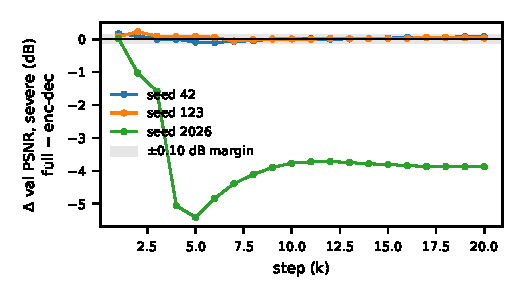
\includegraphics[width=\linewidth]{fig_severe_gap.pdf}
\caption{Validation severe-damage PSNR difference, full model minus encoder--decoder, for the converged seeds
(250 validation images, every 1{,}000 steps). Grey band: $\pm$0.10\,dB equivalence margin.}
\label{fig:curves}
\end{figure}

\subsection{Baselines (same protocol)}
\IfFileExists{\T{tab_baselines.tex}}{\input{\T{tab_baselines.tex}}}{\pending{baseline table: U-Net, NAFNet,
Restormer under the Stage-3 protocol}}
\pending{baseline results text}.
We do not compare against the released model of Wan et al.~\cite{wan2020bringing}: it was trained on different
data and degradations, so a comparison on our synthetic test set would measure the training data rather than the
architecture, and retraining its multi-stage pipeline under our protocol is beyond this study.
\pending{confirm this decision}

\subsection{Cost}
\input{\T{tab_efficiency.tex}}
Removing the translators halves the parameters (\nParamsFull{}M to \nParamsEncdec{}M) and cuts MACs from
\nMACsFull{} to \nMACsEncdec{} GMACs at $256^2$; latency falls by \nLatCut\%, throughput rises by \nThrGain\%,
training time per step falls by \nStepCut\% and peak training memory by \nMemCut\% (Table~\ref{tab:efficiency}).

\subsection{Real photographs (qualitative)}
\begin{figure}[t]
\centering
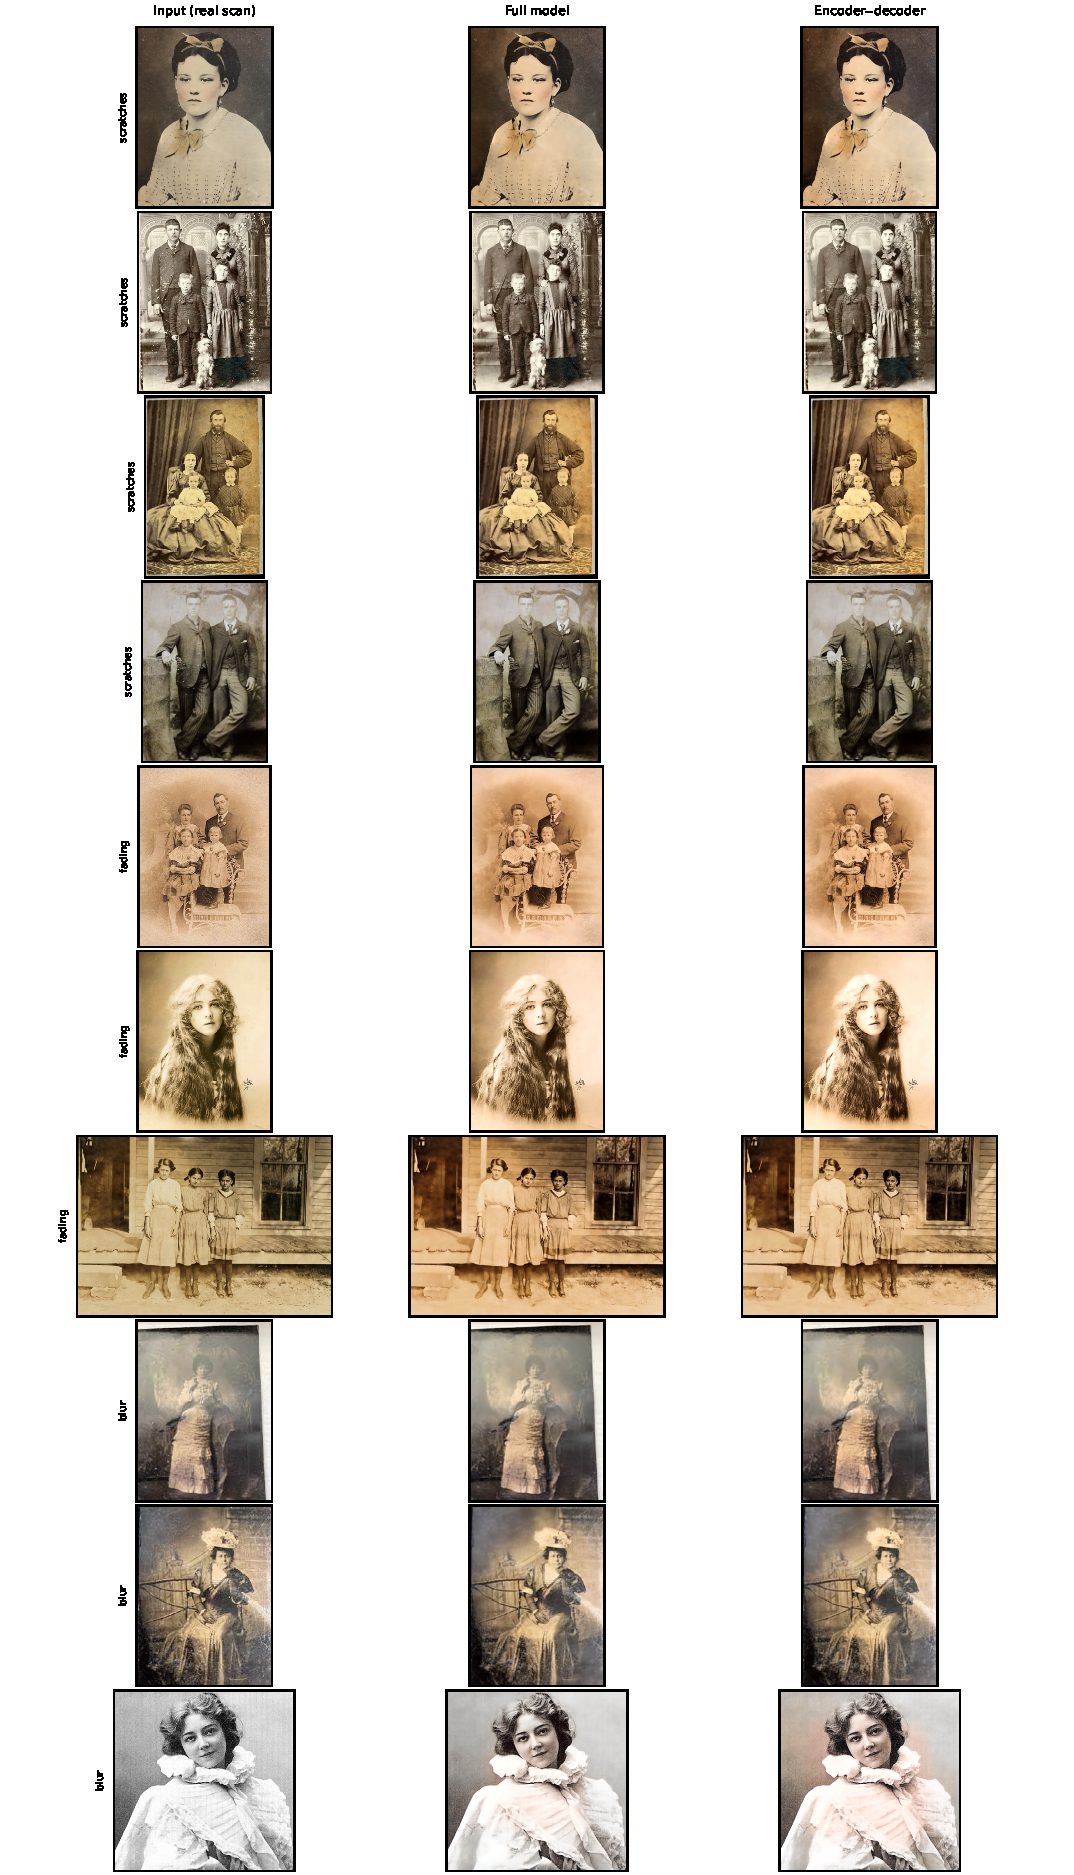
\includegraphics[width=\linewidth]{fig_real_panel.pdf}
\caption{Real scanned photographs (no ground truth; models trained only on synthetic degradation; seed 42, 20k
steps). The ten photos and their damage categories were fixed from the inputs before any model was run.
Quantitative results (Tables~\ref{tab:gating}--\ref{tab:converged}) are on synthetic degradation only.}
\label{fig:real}
\end{figure}
On real scans (Fig.~\ref{fig:real}) neither model visibly removes scratches, tears or spots; both mainly raise
contrast and saturation and add a warm cast, and the two models' outputs are nearly indistinguishable. The
synthetic training degradation does not transfer to these photographs.

\section{Discussion}
\textbf{Budget changes the answer.} At 800 steps the smaller encoder--decoder learns faster and comes out ahead;
with 25$\times$ more training the full model catches up and, in the runs that converged, gains a small
severe-damage advantage in SSIM and LPIPS but not PSNR. Short-budget ablations can confuse faster optimisation with
better final capability.
\textbf{Is the gain worth it?} The converged severe-damage gain is small (LPIPS \nSevLPIPSgain{}) against
\nParamRatio$\times$ the parameters, \nMACsRatio$\times$ the MACs, higher latency, longer training, and a failed
run in one of three seeds. For mild and medium damage, or when training reliability and cost matter, the
encoder--decoder is the better choice on current evidence; translators are a compute-for-quality trade-off only on
heavily damaged inputs.
\textbf{Conditioning.} An oracle that knows the true damage adds less than 0.1\,dB through the gate pathway,
suggesting that this backbone infers the degradation implicitly; conditioning inside the translator blocks was not
tested.

\section{Limitations}
(1)~\textbf{Training budget.} 20k steps is short: both models were still improving, and the full model's
severe-damage lead was still widening at the end, so the size of the converged gap is not known.
(2)~\textbf{Two clean seeds for the full model.} The converged-run analysis rests on seeds \nConvSeeds{}; the
divergence criterion (validation drawdown above \nDivThreshold{}~dB) was fixed after observing the runs.
(3)~\textbf{Unknown cause of divergence.} \pending{update from diagnostic}. Whether a stabiliser (e.g.\ a lower
learning rate or longer warm-up) would remove the instability without changing the comparison is untested.
(4)~\textbf{Synthetic degradation.} Training and test use the same synthetic pipeline on one dataset of mostly
portraits; on real photographs neither model visibly repairs damage, and no real test set with ground truth was
used.
(5)~\textbf{Dataset provenance.} \pending{licence and source of the training images}.
(6)~\textbf{Scope.} Gating was tested only at the short budget; margins were chosen by the authors; timing comes
from one Apple GPU in FP32.

\section{Conclusion}
Under one controlled protocol, damage-conditioned gating gives no benefit to this old-photo restoration backbone,
even with oracle damage information. Latent translators give no benefit at a short budget and, at a longer budget
and only in runs that converged, a small severe-damage SSIM/LPIPS gain without a PSNR gain, at about twice the
parameters and with less stable training. Claims about restoration modules should be checked at more than one
budget, per training run, and against their cost.

\section*{Acknowledgment}
\pending{funding / thanks}. AI assistance: an AI coding assistant (Claude, Anthropic) was used to write and review
experiment and analysis code, to generate the tables and figures from the stored results, and to help draft and
edit the text. All experiments were run, and all results checked, by the authors, who take full responsibility for
the content.

\bibliographystyle{IEEEtran}
\bibliography{refs}

\end{document}
